\section{Method}
\label{sec:method}

\subsection{Hypotheses}
The hypotheses were stated in the research proposal before any player data were collected (Table~\ref{tab:hyp}). RQ4 is descriptive and has no hypothesis.

\begin{table}[ht]
\centering
\caption{Hypotheses and the tests that decide them.}
\label{tab:hyp}
\small
\begin{tabular}{l>{\raggedright\arraybackslash}p{8.2cm}>{\raggedright\arraybackslash}p{4.6cm}}
\toprule
 & Statement & Test \\
\midrule
H0 & Players are born in proportion to births: every area produces players at its expected rate. & Inhomogeneous $L$-function; EB Moran's $I$ \\
H1 & Some areas produce significantly more (hotspots) or fewer (coldspots) players than births predict. & Getis-Ord $G_i^*$, LISA with FDR control \\
H2 & Production is associated with deprivation, urbanisation and proximity to professional clubs and academies. & Negative binomial and spatial regression coefficients \\
\bottomrule
\end{tabular}
\end{table}

\subsection{Expected counts and the standardised ratio}
For area $i$ with $B_{iy}$ male births in year $y$, the expected number of players is
\begin{equation}
E_i = \sum_{y=1975}^{2005} B_{iy}\, \frac{O_{y}}{B_{y}},
\end{equation}
where $O_y$ and $B_y$ are the numbers of mapped players and of male births in England in year $y$. The standardised ratio is $\mathrm{SR}_i = O_i/E_i$, so an SR of 2 means twice as many players as births predict. By construction $\sum_i O_i = \sum_i E_i$. Small areas give unstable ratios, so for mapping and local tests we shrink each SR towards the England rate with the Poisson Empirical Bayes estimator \cite{marshall1991} (SR$_{EB}$).

\subsection{Areas}
\label{sec:units}
A footballer's recorded birthplace is usually the town of the maternity hospital, which is not necessarily where he grew up. Local authorities with a large maternity hospital therefore appear as hotspots and the districts around them as coldspots (Figure~\ref{fig:hospital}). In Oxfordshire, for example, Oxford has an SR of \oxfSR{} and the four surrounding districts between \oxfNbLo{} and \oxfNbHi{}; taken together the five give \oxfAll{}. Travel to Work Areas (TTWAs) are built from commuting flows and normally contain both a hospital town and its catchment, so we use the \nTTWA{} English TTWAs (2011 definition \cite{onsgeo}) as the main areas. The \nLAD{} local authorities and \nHexTwenty{} hexagons of 20\,km are robustness checks; at 10\,km, \zeroHexTen\% of hexagons have no player, which is too sparse. Wikidata places every ``London'' birthplace at a single point in Westminster, so the \nLondonOnly{} ``London'' players are counted only at TTWA level, where London is one area. The median expected count is \medETTWA{} per TTWA, \medELAD{} per local authority and \medEHex{} per 20\,km hexagon; \smallTTWA{} TTWAs expect fewer than five players.

\begin{figure}[ht]
\centering
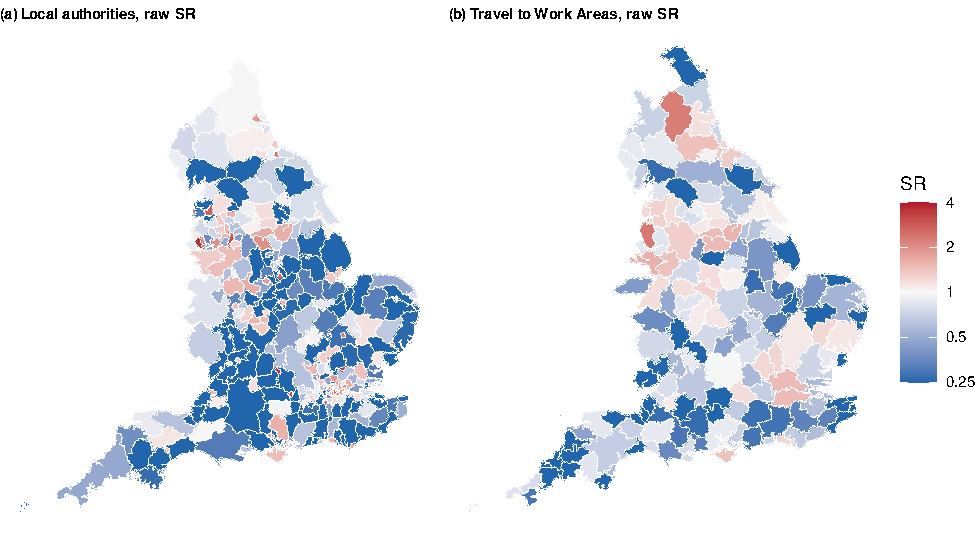
\includegraphics[width=\textwidth]{figures/fig_hospital.pdf}
\caption{Raw standardised ratio by local authority (a) and by Travel to Work Area (b). At local-authority level, towns with large maternity hospitals stand out from the districts around them; TTWAs merge them. Values below 0.25 are shown as 0.25.}
\label{fig:hospital}
\end{figure}

\subsection{RQ1: clustering beyond births}
\paragraph{Regions} We compare the nine English regions with exact Poisson tests of $O = E$.

\paragraph{Point pattern} The inhomogeneous $L$-function \cite{baddeley2000,baddeley2015} measures whether points are closer to each other than expected given a varying background intensity. The background is male births 1975--2005, shared from local authorities to LSOA centroids and kernel-smoothed ($\sigma = 2$\,km), scaled to the number of players. We use the \nTown{} town-level birthplaces, border edge correction and distances up to 60\,km; beyond that the border correction leaves too few points in a country as narrow as England. We simulate \nSim{} patterns of the same size from the births intensity and report the global maximum absolute deviation (MAD) and Diggle-Cressie-Loosmore-Ford (DCLF) tests over 0--60\,km and over 20--60\,km, which leaves out the short distances most affected by shared town coordinates and maternity hospitals. As a check that the method does not create clustering, we apply the same tests to one pattern drawn from births alone, with 199 simulations.

\subsection{RQ2: hotspots and coldspots}
Global clustering of SR$_{EB}$ is tested with the Empirical Bayes Moran's $I$ \cite{assuncao1999} and \nSim{} permutations. Neighbours share a border (TTWAs and local authorities; the Isle of Wight and the Isles of Scilly are linked to their nearest area) or are the 6 nearest areas; for hexagons, the 4, 6 or 8 nearest. Local clusters are located with the Getis-Ord $G_i^*$ \cite{getis1992} (binary weights including the area itself) and local Moran's $I$ (LISA) \cite{anselin1995}, each with \nPerm{} conditional permutations. With 155 areas, 999 permutations cannot reach the $p$-value that a false discovery rate (FDR) correction would need, hence the larger number. We control the FDR across areas with the Benjamini-Hochberg procedure \cite{benjamini1995} and report three tiers: $q<0.05$, $q<0.10$ and unadjusted $p<0.05$ (exploratory). Because the SR distribution is skewed, the permutation test is the main result and the normal approximation a sensitivity analysis.

\subsection{RQ3: explaining the differences}
\label{sec:models}
For TTWA $i$ we fit negative binomial models \cite{venables2002}
\begin{equation}
\log \mathbb{E}[O_i] = \log E_i + \beta_0 + \beta_1\,\mathrm{IMD}_i/10 + \beta_2\,\mathrm{Urban}_i/10 + \beta_3\,\mathrm{Dist}_i/10 \;\bigl[+\; \gamma_{r(i)}\bigr],
\end{equation}
with the IMD score in units of 10 points, the urban share in units of 10 percentage points and the distance in units of 10\,km. M1 has no region term; M2, the main model, adds fixed effects for the region $r(i)$ that holds most of the TTWA's population. Coefficients are reported as rate ratios $e^{\beta}$ with Wald 95\% confidence intervals. We check overdispersion against a Poisson model, collinearity with variance inflation factors, and residual spatial autocorrelation with Moran's $I$ on the Pearson residuals (999 permutations). Lagrange multiplier tests \cite{anselin1988} decide whether a spatial error or spatial lag model is needed; both are also fitted (\texttt{spatialreg} \cite{bivand2015}) on $\log \mathrm{SR}_{EB,i}$ with the same covariates and region effects.

\paragraph{Robustness} M2 is refitted on eight variants of the data: certain evidence only, Premier League players only, the 1975--89 and 1990--2005 birth cohorts separately, without season-ambiguous players, with the total population instead of male births as baseline, without the TTWAs of the five largest cities, and on local authorities instead of TTWAs.

\paragraph{Academy-era sub-model} The Elite Player Performance Plan created Category 1 academies in 2012. For the \nAcadPlayers{} English-born players born 1996--2005 we compute the distance to the nearest Category 1 academy (from 2012/13) and to the nearest club in the season each cohort turned 12 (for cohorts that turned 12 before 2012/13, the 2012/13 academies are used) and fit three models that also include deprivation, urban share and region effects: club distance (A1), academy distance (A2) and both (A3).

\subsection{RQ4: players born outside England}
We count study players by country of birth (England, Scotland, Wales and Northern Ireland separately) and birth cohort, and divide by the country's mean population over 1975--2005 to get players per million people. Countries are grouped by continent.
